\newpage
\section{Polares da aeronave}\label{sec:polares}

As polares foram levantadas em $M = 0{,}85$ com a incidência de empenagem
da Seção 4, varrendo metas de $C_L$ de $-0{,}5$ até o
$C_{L\mathrm{max}}$ do método da seção crítica de cada caso. Foram
avaliadas quatro configurações: CG dianteiro e traseiro, cada um sem
deflexão de superfícies de controle e com a arfagem compensada
($C_M = 0$ pelo profundor). O ponto de projeto está marcado com um losango
em todas as curvas.

\begin{figure}[H]
\centering
\caption{Polar de arrasto das quatro configurações. O losango marca o
ponto de projeto.}\label{fig:polar}
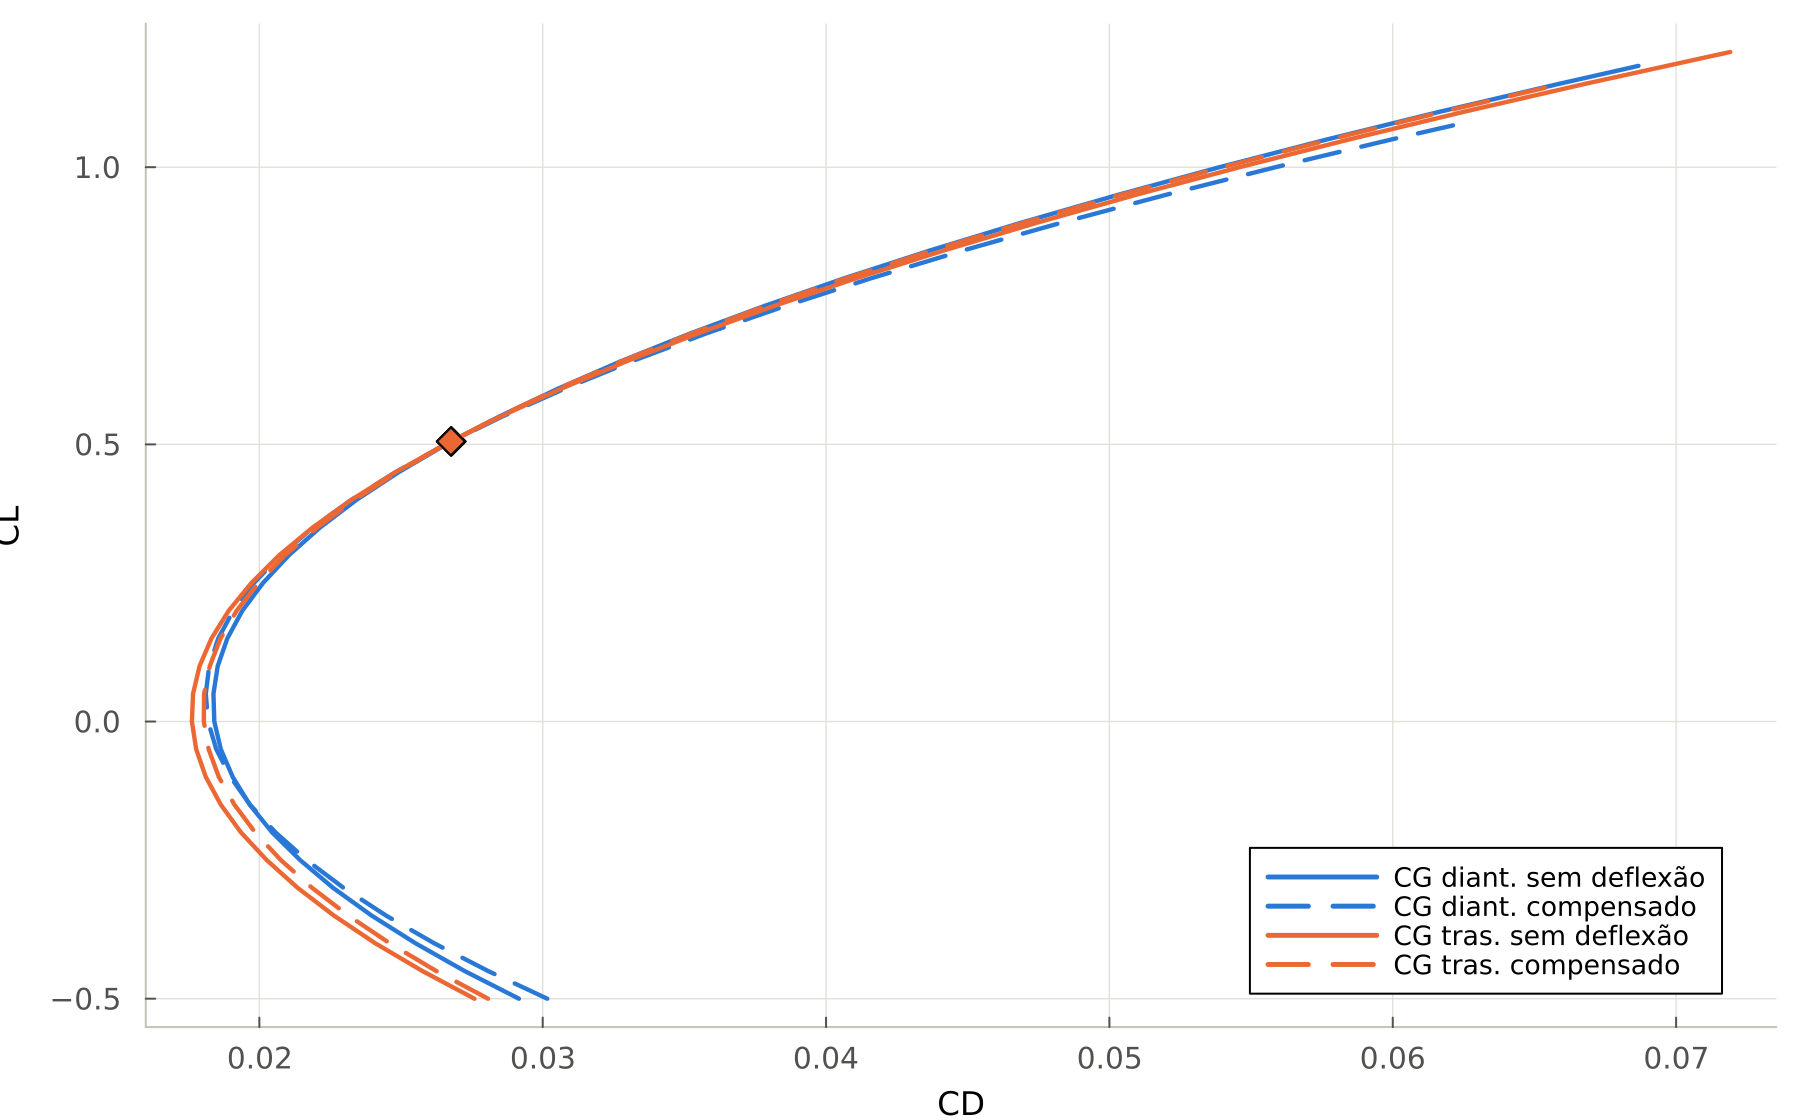
\includegraphics[width=0.9\linewidth]{images/06_polares/polar_cd_cl.png}
\end{figure}

\begin{table}[H]
\centering
\caption{$C_D$ no $C_L$ de projeto para cada configuração e comparação com o \texttt{designTool}.}\label{tab:cd_projeto}
\renewcommand{\arraystretch}{1.25}
\begin{tabular}{lcc}
\toprule
Configuração & $C_D$ em $C_L = 0{,}5053$ & Desvio do \texttt{designTool} \\
\midrule
CG dianteiro sem deflexões & 0,02678 & $+11{,}3\%$ \\
CG dianteiro compensado ($C_M = 0$) & 0,02678 & $+11{,}3\%$ \\
CG traseiro sem deflexões & 0,02676 & $+11{,}2\%$ \\
CG traseiro compensado ($C_M = 0$) & 0,02676 & $+11{,}2\%$ \\
\texttt{designTool} (polar do Lab 02) & 0,02407 & referência \\
\bottomrule
\end{tabular}
\end{table}

No ponto de projeto os casos com e sem compensação coincidem, porque a
incidência da empenagem foi ajustada justamente para zerar o profundor
nessa condição. Com a torção otimizada, as duas posições de CG passam a
apresentar praticamente o mesmo arrasto de projeto, a menos de meio ponto,
sinal de que o washout equilibrou o carregamento de forma robusta à
posição do CG. O arrasto do AVL fica cerca de 11\% acima do
\texttt{designTool}, diferença que vem do arrasto induzido do modelo, que
inclui a contribuição da empenagem carregada e da força de compensação,
enquanto a polar do \texttt{designTool} assume o fator de Oswald da asa
isolada.

\subsection*{Curvas de sustentação}

\begin{figure}[H]
\centering
\caption{Curvas de sustentação das quatro configurações. O losango marca o
ponto de projeto.}\label{fig:cl_alpha}

\includegraphics[width=0.9\linewidth]{images/06_polares/cl_alpha.png}
\end{figure}

As curvas dos dois CGs praticamente coincidem dentro de cada condição de
compensação: a inclinação $C_{L\alpha}$ não depende da posição do CG. A
compensação reduz levemente a sustentação disponível em ângulos altos no
CG dianteiro, coerente com a discussão do $C_{L\mathrm{max}}$.

\subsection*{Deflexão de profundor}

\begin{figure}[H]
\centering
\caption{Deflexão de profundor das quatro configurações. Os casos sem
deflexão aparecem como retas verticais em $\delta_e = 0$. O losango marca
o ponto de projeto.}\label{fig:cl_de}
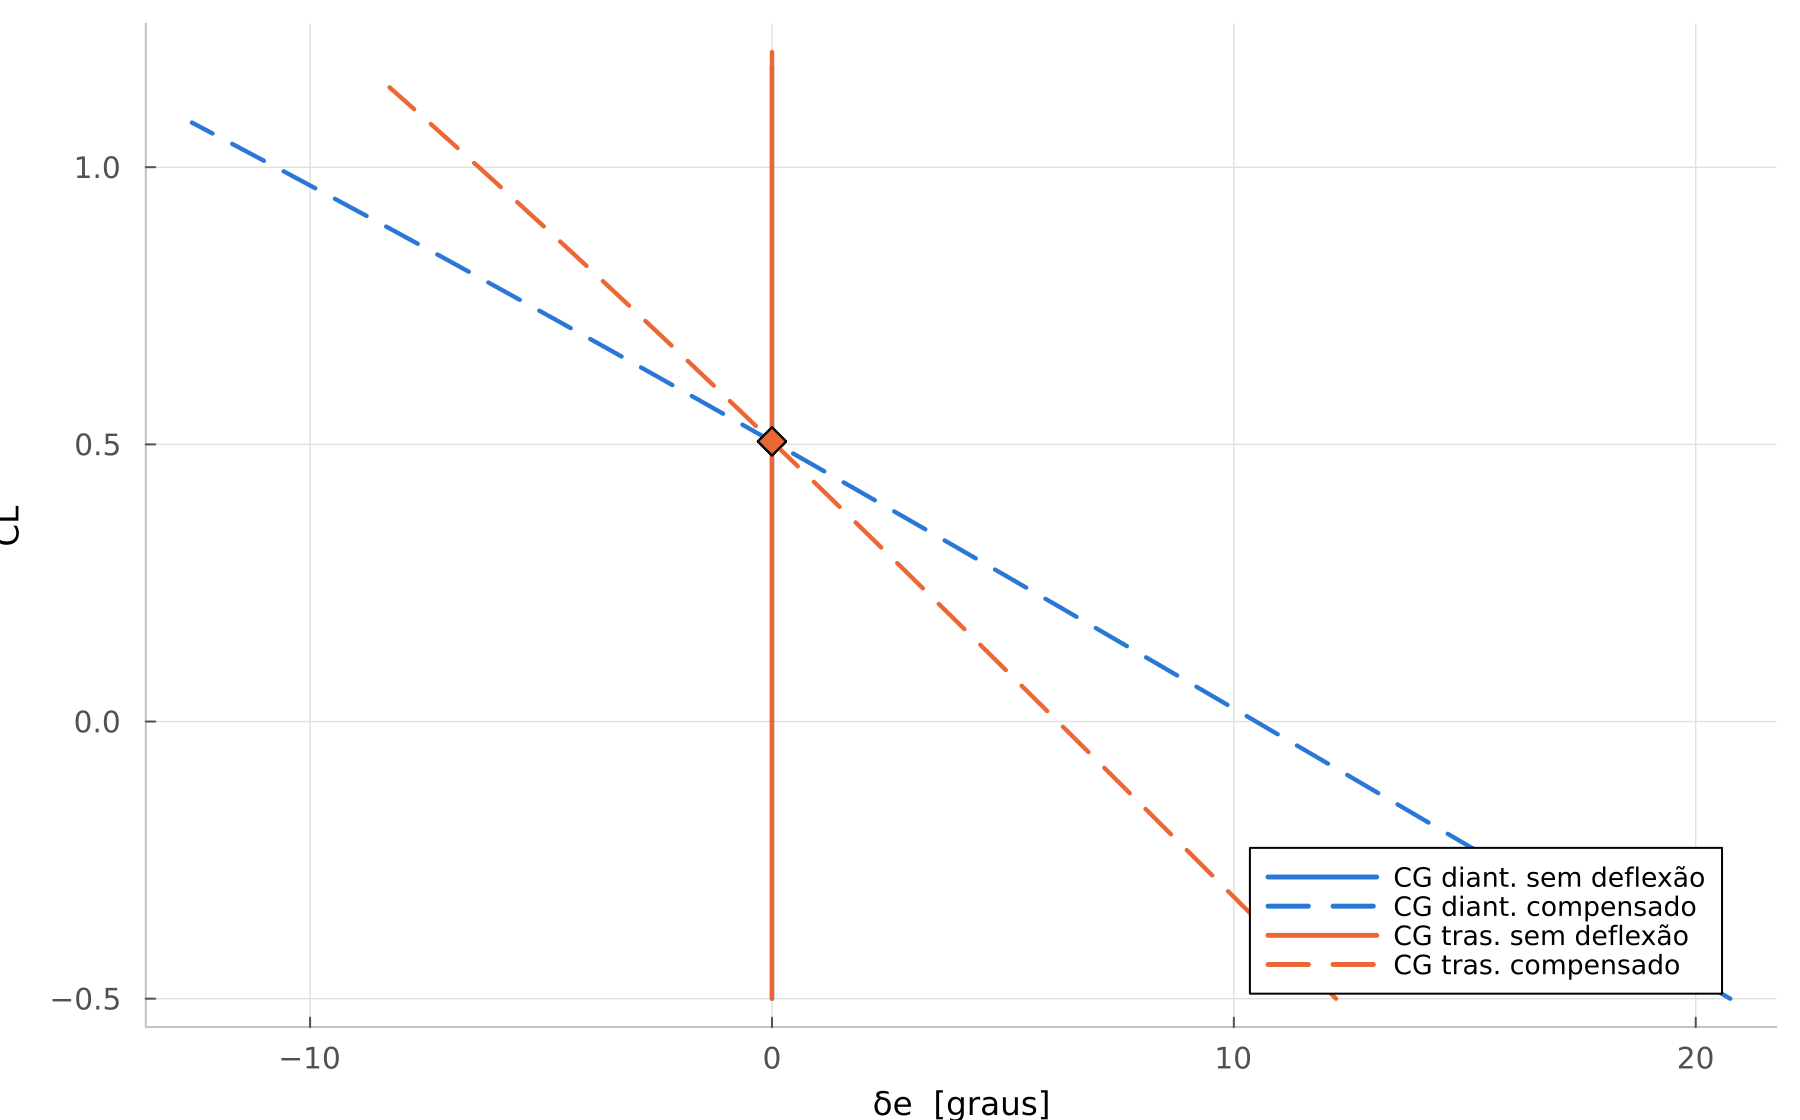
\includegraphics[width=0.9\linewidth]{images/06_polares/cl_de.png}
\end{figure}

Nos casos compensados, o profundor varre de $-12{,}6^\circ$ no
$C_{L\mathrm{max}}$ a $+20{,}7^\circ$ no $C_{L\mathrm{min}} = -0{,}5$ para
o CG dianteiro, e de $-8{,}3^\circ$ a $+12{,}2^\circ$ para o traseiro,
cruzando o zero no ponto de projeto. O gradiente é mais forte no CG
traseiro porque a margem estática menor exige menos momento por unidade de
$C_L$, mas a autoridade por grau de profundor é a mesma. As deflexões
ficam dentro de batentes típicos de profundor ($\pm 25^\circ$), portanto
em níveis adequados na faixa de voo útil, embora o extremo de
$C_{L\mathrm{min}}$ no CG dianteiro já consuma boa parte do batente e o
conjunto incidência mais deflexão trabalhe longe do neutro pelas razões
discutidas na Seção 4.
